\documentclass[12pt, a4paper]{article}

% ── Paquetes ────────────────────────────────────────────────────────────────
\usepackage[utf8]{inputenc}
\usepackage[T1]{fontenc}
\usepackage[spanish]{babel}
\usepackage{geometry}
\usepackage{amsmath}
\usepackage{amssymb}
\usepackage{booktabs}
\usepackage{array}
\usepackage{longtable}
\usepackage{hyperref}
\usepackage{graphicx}
\usepackage{xcolor}
\usepackage{fancyhdr}
\usepackage{titlesec}
\usepackage{parskip}
\usepackage{setspace}
\usepackage{enumitem}
\usepackage{placeins}
\usepackage{makecell}
\usepackage{caption}

% ── Geometría ───────────────────────────────────────────────────────────────
\geometry{
  top=2.5cm,
  bottom=2.5cm,
  left=3cm,
  right=2.5cm
}

% ── Colores UNAM ────────────────────────────────────────────────────────────
\definecolor{unamblue}{RGB}{0, 51, 102}
\definecolor{unamgold}{RGB}{200, 160, 0}
\definecolor{lightgray}{RGB}{245, 245, 245}

% ── Configuración de hyperref ───────────────────────────────────────────────
\hypersetup{
  colorlinks=true,
  linkcolor=unamblue,
  urlcolor=unamblue,
  citecolor=unamblue,
  pdftitle={Proyecto Final - Nexus Sentinel: Deteccion de Uso Indebido de Credenciales},
  pdfauthor={Arellano Ortiz Andre}
}

% ── Encabezado y pie de página ──────────────────────────────────────────────
\pagestyle{fancy}
\fancyhf{}
\fancyhead[L]{\small\textcolor{unamblue}{Nexus Sentinel --- Detección de Uso Indebido de Credenciales}}
\fancyhead[R]{\small\textcolor{unamblue}{UNAM --- Ciencia de Datos G33}}
\fancyfoot[C]{\thepage}
\renewcommand{\headrulewidth}{0.4pt}
\renewcommand{\headrule}{\hbox to\headwidth{\color{unamblue}\leaders\hrule height \headrulewidth\hfill}}

% ── Secciones ───────────────────────────────────────────────────────────────
\titleformat{\section}{\large\bfseries\color{unamblue}}{\thesection.}{0.5em}{}
\titleformat{\subsection}{\normalsize\bfseries\color{unamblue}}{}{0em}{\thesubsection\quad}
\titleformat{\subsubsection}{\normalsize\itshape\color{unamblue}}{}{0em}{\thesubsubsection\quad}

% ── Espaciado ───────────────────────────────────────────────────────────────
\setlength{\parskip}{6pt}
\setlength{\parindent}{0pt}
\onehalfspacing

\captionsetup{font=small, labelfont={bf,color=unamblue}}

% ────────────────────────────────────────────────────────────────────────────
\begin{document}

% ============================================================================
%  PORTADA  (se conserva el formato del módulo previo; los datos se ajustarán)
% ============================================================================
\begin{titlepage}
  \thispagestyle{empty}

  % Línea superior de color
  \noindent\makebox[\linewidth]{\color{unamblue}\rule{\paperwidth}{4pt}}
  \vspace{0.3cm}

  % Institución
  \begin{center}
    {\LARGE\bfseries\color{unamblue}
      Universidad Nacional Autónoma de México}\\[0.3cm]
    {\large\color{unamblue} Facultad de Estudios Superiores Acatlán}\\[1.2cm]

    % Línea decorativa
    \textcolor{unamgold}{\rule{0.6\textwidth}{1.5pt}}\\[1.2cm]

    % Diplomado
    {\Large\bfseries\color{unamblue} Diplomado en Ciencia de Datos}\\[0.2cm]
    {\large\color{unamblue} Generación 33}\\[1.5cm]

    % Título del proyecto
    \textcolor{unamgold}{\rule{0.6\textwidth}{1.5pt}}\\[1cm]
    {\huge\bfseries\color{unamblue} Proyecto Final}\\[0.3cm]
    {\LARGE\bfseries Nexus Sentinel}\\[0.5cm]
    \textcolor{unamgold}{\rule{0.6\textwidth}{1.5pt}}\\[1cm]

    % Subtítulo
    {\large\itshape Detección de uso indebido de credenciales mediante analítica
     de comportamiento de usuarios y entidades (UEBA)}\\[2cm]

    % Datos del proyecto
    \begin{tabular}{rl}
      \textbf{Presentado a:} & Raúl López Benítez \\[0.4cm]
      \textbf{Autor:}        & Arellano Ortiz Andre \\[0.4cm]
      \textbf{Fecha:}        & 24 de julio del 2026 \\
    \end{tabular}

    \vfill

    % Línea inferior de color
    \textcolor{unamgold}{\rule{0.6\textwidth}{1.5pt}}\\[0.5cm]
    {\small\color{gray} Ciudad de México, México}
  \end{center}

  \vspace{0.3cm}
  \noindent\makebox[\linewidth]{\color{unamblue}\rule{\paperwidth}{4pt}}
\end{titlepage}

% ============================================================================
%  CUERPO DEL DOCUMENTO
% ============================================================================
\newpage
\tableofcontents
\newpage

% ────────────────────────────────────────────────────────────────────────────
\section{Introducción}

El perímetro de seguridad tradicional ---firewall, antivirus, sistemas de detección de
intrusiones--- fue diseñado para detener a un intruso que \textit{rompe} algo. Sin embargo, la
mayoría de las brechas modernas no rompen nada: utilizan \textbf{credenciales legítimas}, robadas
mediante \textit{phishing}, compradas en mercados ilícitos o abusadas por un empleado, para moverse
dentro de la red como si fueran un usuario normal. Este es el problema que la industria denomina
UEBA (\textit{User and Entity Behavior Analytics}) y que, en la práctica, resulta indistinguible de
la amenaza interna: en ambos casos el atacante opera dentro de canales autorizados y cada
autenticación individual es, técnicamente, válida.

En este proyecto desarrollé \textbf{Nexus Sentinel}, un sistema de puntuación de riesgo que detecta
este tipo de comportamiento sobre datos reales de autenticación de una red corporativa. Concebí el
proyecto en torno a una premisa que gobernó todas mis decisiones de diseño: \textit{el modelo no debe
ver eventos, sino desviaciones}. Una autenticación aislada no dice nada; lo que delata a una cuenta
comprometida es la desviación de su patrón de comportamiento habitual. A lo largo del documento
narro, en primera persona, el desarrollo completo: desde la adquisición de mil millones de eventos
crudos hasta el despliegue de una interfaz funcional en producción, pasando por la ingeniería de
variables ---que considero el corazón técnico del trabajo--- y una evaluación que me esforcé por
mantener honesta incluso cuando los resultados no fueron los que esperaba.

La tarea que abordo es de \textbf{clasificación binaria supervisada} sobre la unidad de análisis
\textbf{usuario-día}: dado el resumen del comportamiento de autenticación de un usuario durante un
día, el sistema debe estimar la probabilidad de que ese día contenga actividad de compromiso. El
problema presenta los retos estructurales que definen a la ciencia de datos aplicada a la
ciberseguridad: un desbalance de clases extremo (menos del 0.4\% de los casos son positivos), un
volumen masivo de datos (más de mil millones de eventos), datos desidentificados por privacidad y la
necesidad de que el resultado sea \textit{explicable}, pues ninguna acción sobre una cuenta o una
persona puede tomarse a ciegas.

\subsection{La empresa y su propuesta de valor}

\textbf{Nexus Sentinel} es la empresa ficticia de analítica de seguridad que constituí para este
proyecto. Su producto es precisamente el sistema que documento aquí: una capa de inteligencia que
las organizaciones incorporan sobre su infraestructura de seguridad existente para detectar el uso
indebido de credenciales legítimas.

El escenario que Nexus Sentinel resuelve es el siguiente. Una empresa cliente sufre un incidente en
el que la cuenta de uno de sus ingenieros es utilizada durante semanas para explorar servidores a
los que ese ingeniero jamás accedía. Ninguna alerta se dispara, porque cada autenticación individual
es «válida», y el incidente se detecta tarde y de forma casi accidental. Como muestro en la
presentación del proyecto, este escenario tiene equivalentes reales y costosísimos en la industria
---el caso más conocido es el de Target en 2013, donde la credencial robada a un proveedor externo
condujo a una brecha de más de 200 millones de dólares.

Ese es el problema que Nexus Sentinel ataca: no vigilar eventos individuales, sino la
\textbf{desviación del patrón de comportamiento} de cada cuenta. En este documento desarrollo el
producto de principio a fin, validándolo sobre datos reales de una red corporativa.

\subsection{Flujo de trabajo}

El desarrollo comprende siete etapas encadenadas: la adquisición y el muestreo justificado de los
datos crudos; un análisis exploratorio orientado a descubrir empíricamente las señales de compromiso;
la ingeniería de variables en cuatro niveles de desviación; el modelado supervisado y no supervisado
con su evaluación y análisis de estabilidad; la construcción del flujo de inferencia y la puntuación
de riesgo; la exposición de los modelos mediante una API; y el desarrollo de una interfaz web con un
asistente conversacional.

Cerré cada etapa con una verificación explícita, y varias de ellas revelaron conflictos técnicos y
metodológicos que documento con transparencia, pues considero que la forma en que los resolví es
parte sustancial del valor del trabajo.

% ────────────────────────────────────────────────────────────────────────────
\section{Planteamiento del problema}

La analítica de comportamiento de usuarios y entidades parte de una observación empírica bien
documentada: el uso de credenciales robadas o abusadas es uno de los vectores más frecuentes en las
brechas de seguridad modernas. El \textit{Data Breach Investigations Report} de Verizon reporta año
con año que el elemento humano y el uso de credenciales comprometidas participan en una fracción
mayoritaria de los incidentes analizados \cite{verizon2024}. La razón es estructural: robar una
credencial es más barato y más silencioso que explotar una vulnerabilidad técnica, y una vez dentro,
el atacante hereda todos los permisos legítimos de la cuenta.

El problema técnico central es que las herramientas perimetrales clásicas ---SIEM, EDR, firewalls---
razonan a nivel de \textit{evento}: una regla se dispara cuando ocurre algo explícitamente
prohibido. Pero el uso indebido de credenciales no viola ninguna regla a nivel de evento: la cuenta
tiene permiso para autenticarse. La señal solo existe a nivel de \textit{patrón}: un usuario que de
pronto se autentica contra decenas de máquinas que jamás había tocado, en horarios inusuales o
mediante protocolos que normalmente no emplea. Detectar esto requiere construir, para cada usuario,
una línea base de comportamiento y medir cuánto se desvía de ella cada día.

\subsection{Decisiones de diseño no negociables}

Antes de escribir una sola línea de código fijé cinco decisiones de diseño que mantuve durante todo
el proyecto, precisamente porque son las que separan una solución operativa de un ejercicio
académico:

\begin{enumerate}[leftmargin=1.5cm]
  \item \textbf{Unidad de análisis = usuario-día.} El riesgo se evalúa sobre el resumen diario del
        comportamiento de cada usuario, no sobre eventos aislados.
  \item \textbf{Métricas para desbalance extremo.} Empleo PR-AUC como métrica rectora, recall a una
        tasa de falsos positivos fija y F1 al umbral operativo. Nunca \textit{accuracy}: con menos
        del 0.4\% de positivos, un clasificador que prediga siempre «normal» acierta el 99.6\% de las
        veces siendo completamente inútil. La literatura respalda esta elección: la curva de
        precisión-recall es más informativa que la ROC al evaluar clasificadores binarios sobre
        conjuntos desbalanceados \cite{saito2015}.
  \item \textbf{Humano en el circuito.} El sistema prioriza y explica; ninguna acción sobre una
        cuenta o una persona es automática. La decisión final siempre es de un analista.
  \item \textbf{Umbrales calibrados por capacidad operativa.} Los umbrales de alerta se fijan por
        percentiles que producen un número de tickets diarios revisable por el equipo de seguridad,
        no mediante números arbitrarios.
  \item \textbf{Muestreo documentado, no oculto.} El volumen masivo se gestiona con un muestreo
        justificado y trazable, jamás escondiendo la reducción de datos.
\end{enumerate}

% ────────────────────────────────────────────────────────────────────────────
\section{Estrategia de negocio}

\subsection{Nicho de negocio}

Posicioné a Nexus Sentinel como una capa de \textbf{UEBA / Human Risk Analytics}: inteligencia
interna para el área de ciberseguridad. La propuesta no compite con el SIEM ni con el EDR, sino que
consume sus registros y devuelve una priorización explicada. La propuesta de valor es medible:
reducir el volumen de alertas que un analista debe revisar manualmente, manteniendo el
\textit{recall} sobre los compromisos reales. En otras palabras, convertir un pajar de mil millones
de eventos en una lista corta, priorizada y justificada de casos investigables.

\subsection{Usuarios finales y accionables}

Diseñé el sistema para tres perfiles de usuario, con el analista de un Centro de Operaciones de
Seguridad (SOC) como usuario principal:

\begin{itemize}[leftmargin=1.5cm]
  \item \textbf{Analista SOC (principal):} necesita una cola priorizada y explicada, no un mar de
        alertas. El sistema le entrega el triaje por riesgo, la explicación de cada caso y las
        acciones de decisión.
  \item \textbf{CISO (secundario):} necesita la tendencia de riesgo organizacional y evidencia para
        justificar inversión. Le entrega un panel ejecutivo con el riesgo agregado y la eficiencia
        del SOC.
  \item \textbf{Oficial de Cumplimiento (implícito):} necesita auditabilidad de las decisiones sobre
        cuentas. Le entrega la trazabilidad completa desde las variables hasta la decisión humana
        registrada.
\end{itemize}

Traduje la puntuación de riesgo (0--100) a tres niveles accionables mediante un semáforo, cuya
correspondencia con las acciones del SOC es uno a uno: \textbf{verde} (registro pasivo que alimenta
la línea base del usuario), \textbf{naranja} (ticket con la evidencia y su explicación, para
revisión) y \textbf{rojo} (investigación prioritaria con validación humana obligatoria antes de
cualquier acción sobre la cuenta).

% ────────────────────────────────────────────────────────────────────────────
\section{Descripción de los datos}

Trabajé con el conjunto de datos \textit{Comprehensive, Multi-Source Cyber-Security Events},
publicado por el Laboratorio Nacional de Los Álamos (LANL) y liberado por su autor para investigación
pública \cite{kent2015data, kent2015book}. Es un conjunto de datos \textbf{reales}: 58 días
consecutivos de eventos desidentificados de la red corporativa interna de LANL, con eventos de un
equipo de \textit{red team} (ataques reales controlados) que sirven como \textit{ground truth} de
comportamiento malicioso. En total, el conjunto documenta 1\,648\,275\,307 eventos de 12\,425
usuarios y 17\,684 computadoras.

Utilicé dos de sus archivos: \texttt{auth.txt.gz} (7.2 GB comprimidos, aproximadamente 1\,051
millones de autenticaciones Windows/Active Directory), que es la fuente principal, y
\texttt{redteam.txt.gz} (4.8 KB), que contiene los eventos de compromiso que uso como etiquetas. Elegí
esta fuente precisamente porque su desbalance extremo, su volumen masivo y su desidentificación
reproducen las condiciones exactas que un científico de datos enfrenta en un SOC real. Cabe destacar
que la guía de la rúbrica veta explícitamente a Kaggle como fuente de datos; LANL es una fuente
institucional primaria y de acceso directo, lo que la hace idónea.

\subsection{Primer conflicto: la adquisición de los datos}

El primer obstáculo real del proyecto apareció en la adquisición. La documentación y los trabajos
previos sobre este conjunto asumen una descarga directa y anónima desde el portal de LANL. Sin
embargo, al momento de desarrollar el proyecto el portal había incorporado un \textit{data fence}:
un formulario que exige un correo electrónico y una declaración de uso, y que a cambio devuelve un
\textit{token} temporal con el que se construye la URL de descarga. Tuve que adaptar mi módulo de
adquisición para solicitar ese token programáticamente antes de poder descargar los archivos, y
documenté la fecha, la URL y el tamaño de cada descarga para garantizar la reproducibilidad.

El segundo obstáculo fue el volumen. Descargar 7.2 GB comprimidos y, sobre todo, procesarlos, exigía
una estrategia cuidadosa: implementé la descarga en \textit{streaming} con reanudación automática
---que efectivamente tuvo que reanudarse tras una interrupción a mitad de la transferencia--- y la
lectura del archivo comprimido por bloques (\textit{chunks}), sin descomprimirlo nunca por completo
a disco. Esta decisión de ingeniería fue la que hizo viable el resto del proyecto en un equipo de
cómputo personal.

\subsection{Muestreo justificado}

Mil millones de eventos ni caben cómodamente en memoria ni son necesarios. Gestioné el volumen con un
muestreo que documenté por completo, en lugar de ocultarlo. Las reglas y su justificación fueron:

\begin{itemize}[leftmargin=1.5cm]
  \item \textbf{Ventana temporal:} los primeros 30 días. Verifiqué empíricamente sobre el archivo
        completo de 58 días que el 100\% de los eventos del \textit{red team} ocurre entre los días 1
        y 29, de modo que la ventana conserva la totalidad del \textit{ground truth}.
  \item \textbf{Usuarios:} incluí las 104 cuentas comprometidas más una muestra aleatoria de 4\,000
        usuarios normales, estratificada por cuartil de actividad y con semilla fija, para no sesgar
        la línea base hacia cuentas hiperactivas ni casi inactivas.
  \item \textbf{Exclusión de cuentas no humanas:} excluí del universo muestreable las cuentas de
        máquina (terminadas en \texttt{\$}) y de sistema (SYSTEM, Local Service, entre otras), pues
        el scoring debe recaer sobre personas.
\end{itemize}

El resultado fue una muestra de 37\,580\,871 eventos para 4\,104 usuarios, que persistí en formato
Parquet (aproximadamente 209 MB) como el conjunto de trabajo reproducible del resto del proyecto.

\subsection{Calidad de los datos}

Documenté las particularidades de calidad de esta fuente real. El campo \texttt{auth\_type} está
ausente (marcado con «\texttt{?}») en el 60.2\% de los eventos, y \texttt{logon\_type} en el 18.7\%.
En lugar de descartar o imputar a ciegas, traté el valor nulo como información en sí mismo, pues su
patrón no es aleatorio sino que depende del mecanismo de recolección de cada evento. Asimismo, el
archivo de \textit{red team} contiene 749 líneas de las cuales 12 líneas distintas aparecen
duplicadas (34 filas en exceso); las deduplico a 715 eventos únicos, correspondientes a 104 cuentas.
Como verificación adicional a nivel de evento, confirmé que 702 de esos 715 eventos tienen su línea
de autenticación exacta en la muestra, y que de esos 702, \textbf{701 fueron autenticaciones
exitosas y solo 1 fue un fallo}. Este dato es una confirmación directa de la tesis del proyecto: el
atacante con credenciales robadas no rompe puertas, las abre.

% ────────────────────────────────────────────────────────────────────────────
\section{Análisis exploratorio de datos}

El objetivo de mi análisis exploratorio fue triple: caracterizar el comportamiento normal de
autenticación, cuantificar el desbalance real y descubrir empíricamente las señales de compromiso que
después convertiría en variables. Adopté un criterio deliberado de presentación: pocas figuras, cada
una respondiendo una pregunta concreta del problema, en lugar de saturar el documento con gráficas
sin valor analítico.

\subsection{El ritmo de la red}

Los tiempos del conjunto son anónimos: son una época que arranca en 1, sin fecha real, por seguridad.
Mi primera pregunta fue si podía recuperar el ritmo humano de la red únicamente a partir de la
periodicidad de los datos. La Figura~\ref{fig:ritmo} muestra que sí. Al agregar los eventos de origen
humano por hora relativa del día (el residuo de dividir el tiempo entre 86\,400 segundos), emerge un
ciclo circadiano claro con un horario laboral inferido de 7:00 a 16:00. Un matiz metodológico
relevante: existe una base de automatización que corre 24/7 bajo cuentas de usuario ---el valle
nocturno conserva cerca del 59\% de la actividad del pico--- por lo que definí la frontera de
«horario laboral» como el punto medio entre el valle y el pico, y no como un porcentaje del pico.
La serie diaria, además, revela los fines de semana sin necesidad de un calendario: aparecen como
caídas de dos días con periodicidad siete. El \textit{red team} ataca en 18 de los 30 días.

\begin{figure}[!htb]
  \centering
  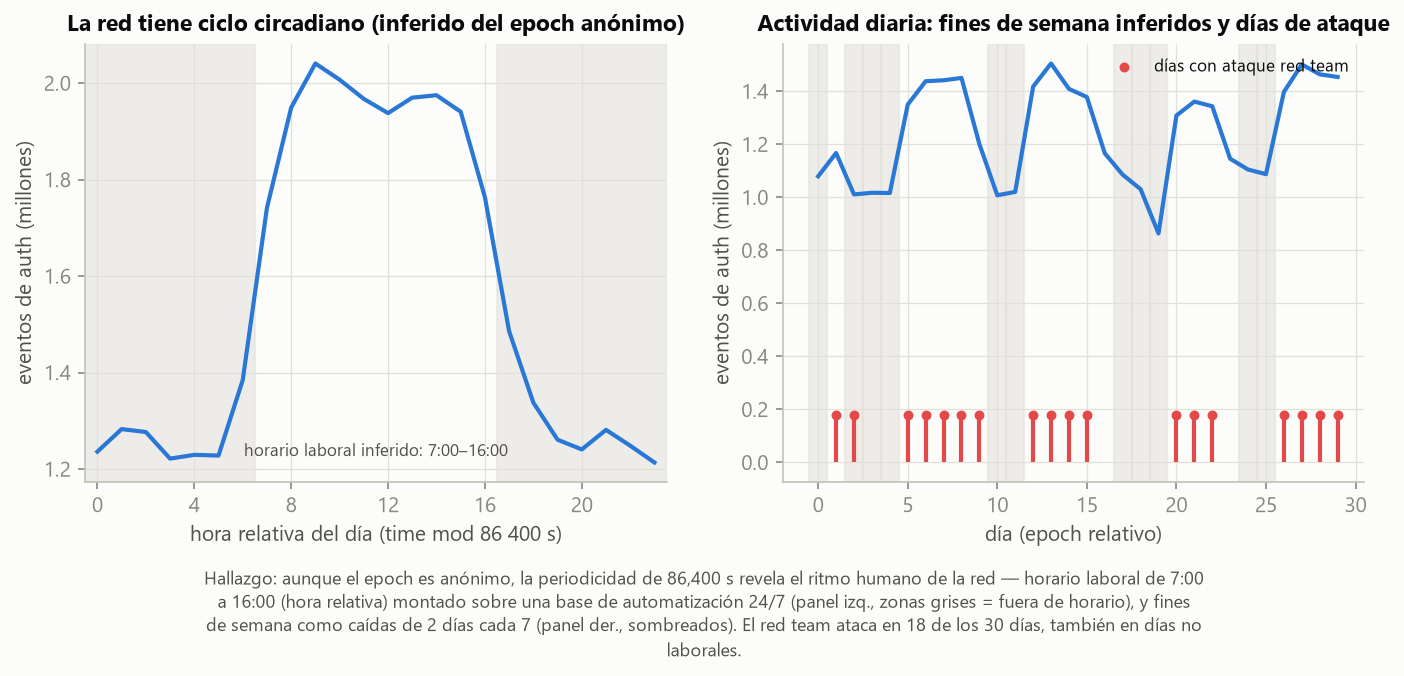
\includegraphics[width=\textwidth]{img/fig1_ritmo_red.png}
  \caption{Ritmo de la red inferido del tiempo anónimo. Izquierda: ciclo circadiano y horario laboral
  inferido (zonas grises = fuera de horario). Derecha: serie diaria con fines de semana sombreados y
  días con ataque marcados en rojo.}
  \label{fig:ritmo}
\end{figure}

\subsection{Las señales del compromiso}

Comparé los 181 usuario-días comprometidos contra los 47\,775 normales sobre tres señales candidatas
(Figura~\ref{fig:senales}). El hallazgo central, y la señal más citada en la literatura sobre este
conjunto, es el \textbf{alcance}: la mediana de computadoras destino distintas es de 22 en los días
comprometidos frente a 10 en los normales ---la huella del movimiento lateral. El segundo hallazgo
fue contraintuitivo y resultó valioso: el compromiso \textbf{no} se parece a un ataque de fuerza
bruta. Los días comprometidos presentan fallos con más frecuencia (50\% de los días frente a 24\%)
pero en proporción mínima (un ratio típico de 0.003), porque quien usa credenciales válidas robadas
avanza con éxito. De hecho, el fallo masivo pertenece a la población normal: el 17\% de los
usuario-días normales son 100\% fallos, la firma de la automatización con credenciales caducas.
Finalmente, el protocolo NTLM ---asociado en la literatura a técnicas de movimiento lateral tipo
\textit{pass-the-hash}, catalogadas por el marco MITRE ATT\&CK \cite{mitre}--- aparece con una
mediana de ratio de 0.02 en los comprometidos frente a 0 en los normales.

\begin{figure}[!htb]
  \centering
  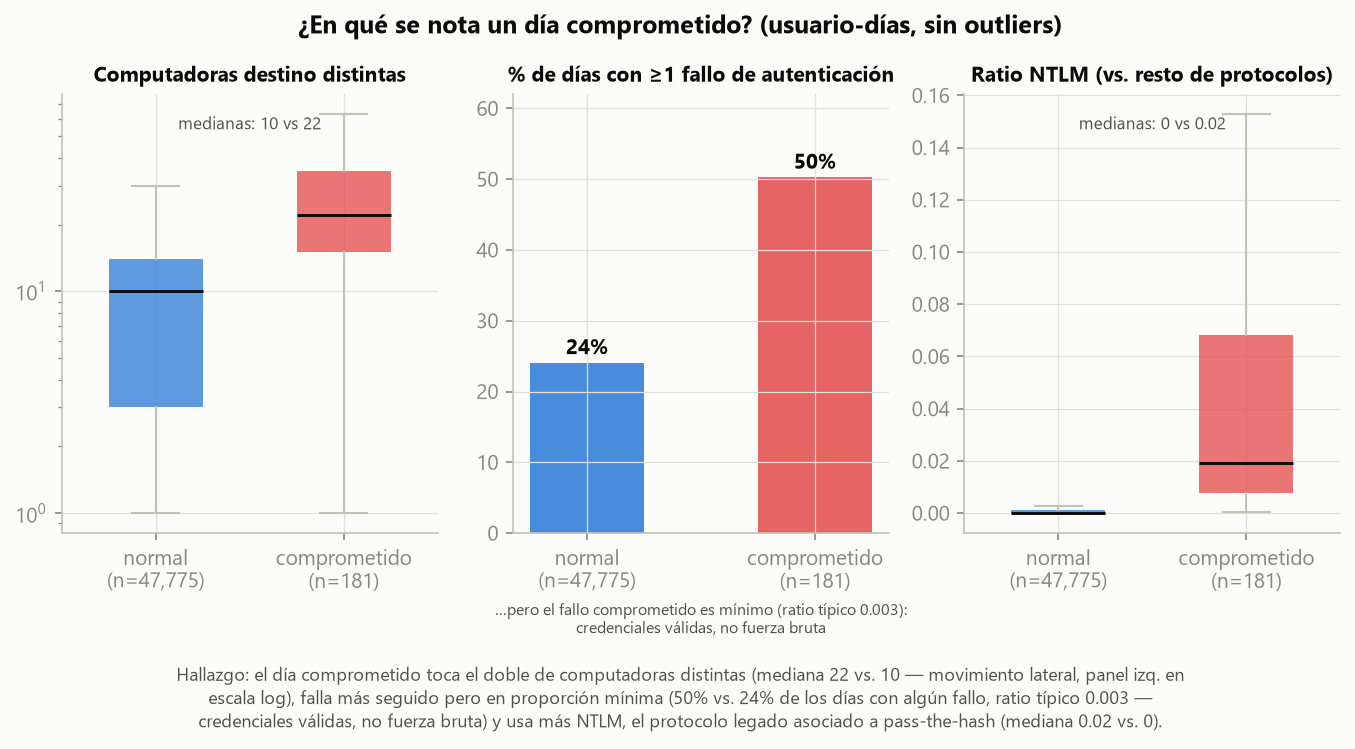
\includegraphics[width=\textwidth]{img/fig2_senales_compromiso.png}
  \caption{Comparación normal vs. comprometido sobre tres señales. El panel de destinos distintos
  hace visible el movimiento lateral; el de fallos revela que el compromiso usa credenciales válidas;
  el de NTLM confirma el protocolo legado como señal.}
  \label{fig:senales}
\end{figure}

\subsection{El movimiento lateral hecho visible}

Para darle una cara concreta al movimiento lateral, construí el grafo de conexiones
usuario$\rightarrow$computadora de una cuenta comprometida, antes y durante el ataque
(Figura~\ref{fig:ego}). En sus ocho días de historia previa, la cuenta acumuló 27 destinos distintos;
el día del ataque tocó 49, de los cuales 28 eran nuevos ---su grafo se expandió más en un solo día
que en toda su historia previa--- y 11 de esos destinos nuevos están confirmados en el
\textit{ground truth}. Ninguna de esas autenticaciones falló ni disparó una alerta tradicional: la
anomalía solo existe a nivel del patrón. Esta figura se convirtió en la «historia visual» del
proyecto y en el prototipo del mini-grafo que después implementé en la interfaz.

\begin{figure}[!htb]
  \centering
  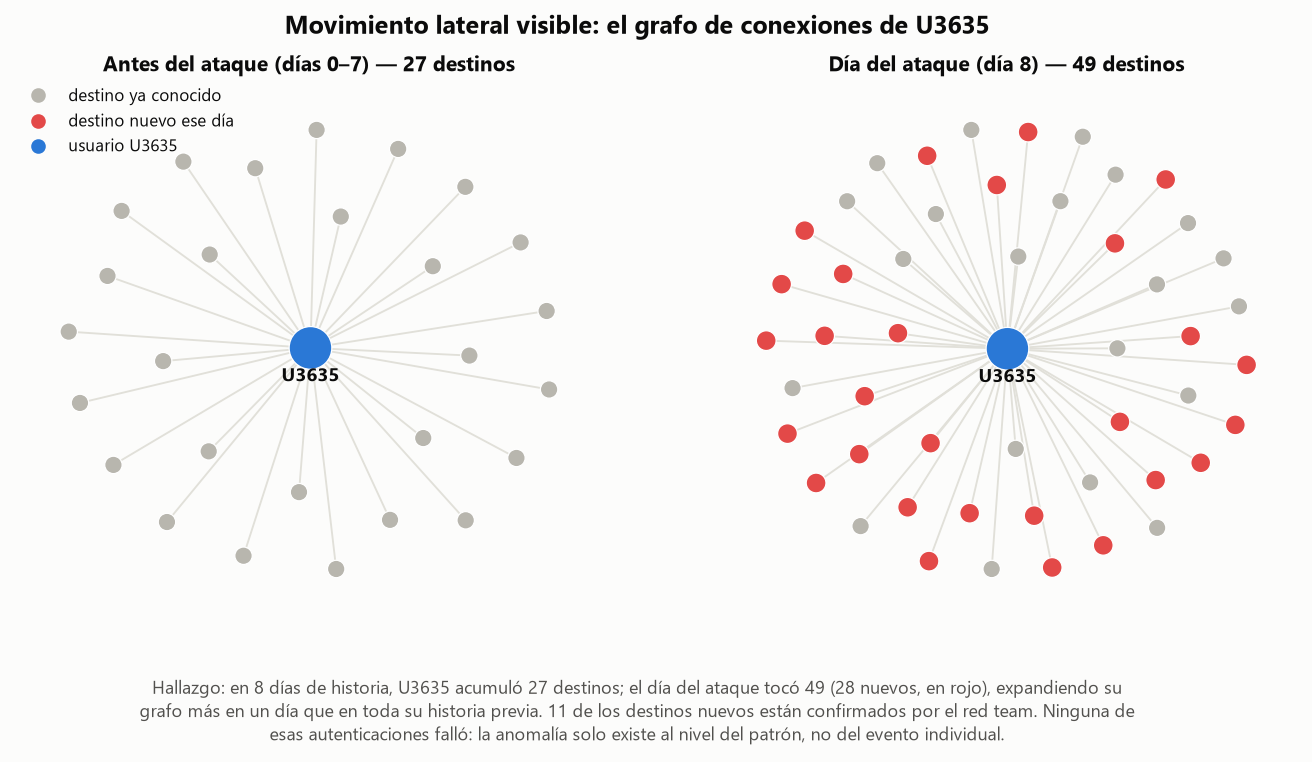
\includegraphics[width=\textwidth]{img/fig3_grafo_ego.png}
  \caption{Grafo ego de una cuenta comprometida. En gris, los destinos que la cuenta ya conocía; en
  rojo, los que tocó por primera vez el día del ataque. El movimiento lateral es la novedad de
  conexiones.}
  \label{fig:ego}
\end{figure}

\subsection{El desbalance}

No presento el desbalance como una gráfica sino como un indicador, porque un número tan extremo se
comunica mejor así: de los 47\,956 usuario-días de la muestra, solo 181 contienen actividad maliciosa
(el 0.38\%, es decir, uno de cada 265), y esto en una muestra deliberadamente enriquecida con la
totalidad de las cuentas comprometidas ---la población real es del orden de 50 veces más
desbalanceada. Este único dato es el argumento definitivo contra el uso de la exactitud como métrica
y la justificación de todas las decisiones de evaluación que tomé después.

% ────────────────────────────────────────────────────────────────────────────
\section{Ingeniería de variables}

Considero esta la sección crítica del proyecto. Mi principio rector fue que cada variable respondiera
una pregunta de desviación, y las organicé en cuatro niveles, donde cada nivel existe porque el
anterior tiene un punto ciego que un atacante disciplinado podría explotar. El resultado es una tabla
maestra de 47\,956 usuario-días descritos por 61 variables, sin valores faltantes ni infinitos.

\begin{itemize}[leftmargin=1.5cm]
  \item \textbf{(a) Variables crudas ---¿qué hizo hoy?} Capturan cada táctica concreta: el
        \textbf{volumen} (número de eventos, logones), el \textbf{alcance} (computadoras destino y
        origen distintas), los \textbf{fallos} (incluida la ráfaga máxima de fallos consecutivos,
        firma de fuerza bruta), el \textbf{protocolo} (conteos de NTLM, Kerberos, tickets TGT/TGS y
        el propio nulo como información), el \textbf{tipo de sesión} y las variables
        \textbf{temporales} que usan las fronteras circadianas inferidas en el EDA.
  \item \textbf{(b) Desviación personal ---¿qué tan distinto de su propio pasado?} Es el corazón del
        proyecto. Para cada variable relevante calculo su z-score respecto a la media histórica del
        propio usuario, su razón contra el máximo histórico y banderas de «primera vez». Lo «normal»
        es personal: 22 destinos son rutina para un administrador y una alarma para un contador.
  \item \textbf{(c) Desviación grupal ---¿qué tan distinto de sus pares?} Resuelve el punto ciego de
        los eventos globales legítimos (una actualización que dispara la actividad de todos). Como los
        datos están desidentificados y no hay roles organizacionales disponibles, construyo los pares
        \textit{conductualmente} mediante agrupamiento (\textit{clustering}) sobre el perfil de cada
        usuario, y mido la desviación del día contra la distribución de su grupo.
  \item \textbf{(d) Novedad de grafo ---¿qué tan nuevo es su grafo de conexiones?} Cierra el punto
        ciego del atacante que mantiene volumen y horario normales pero que, por definición del
        movimiento lateral, no puede evitar tocar máquinas que la cuenta jamás visitó. Calculo el
        número de aristas nuevas, su proporción, la rareza media de los destinos y el número de
        máquinas origen nuevas.
\end{itemize}

\subsection{La regla anti-fuga}

El error metodológico más probable y costoso en un proyecto con partición temporal y variables
históricas es la \textbf{fuga de información} del futuro hacia el pasado. Lo traté como una prioridad
de primer orden y establecí reglas estrictas: toda estadística histórica de la desviación personal se
calcula desplazando la serie del usuario un día (excluyendo el día evaluado de su propia línea base);
el grafo de referencia de la novedad se «congela» al día anterior antes de evaluar cada día; el
modelo de pares se ajusta únicamente con días de entrenamiento; y ninguna variable deriva, directa o
indirectamente, del archivo de etiquetas. Estas reglas las verifiqué explícitamente, línea por línea,
mediante una auditoría dedicada del código.

Como ilustración del poder de este diseño, el día del ataque de la cuenta que analicé en el EDA
presenta un volumen de actividad prácticamente normal (su z-score de volumen es de apenas 0.69, menos
de una desviación estándar), de modo que un detector de volumen no lo vería. Pero las desviaciones de
alcance y novedad lo delatan por completo: tocó destinos a 7.7 desviaciones estándar de su línea base
personal y a 4.5 desviaciones de sus pares conductuales ese mismo día.

\subsection{Etiquetado y partición temporal}

Etiqueté cada usuario-día con \texttt{y = 1} si contiene al menos un evento del \textit{red team},
verificando una cobertura perfecta: los 181 pares (usuario, día) del \textit{ground truth} tienen su
fila correspondiente en la tabla maestra. La partición es \textbf{temporal estricta}, nunca
aleatoria: un \textit{k-fold} aleatorio filtraría información porque los días de un mismo usuario
están autocorrelacionados y las variables históricas cruzarían el corte. Verifiqué además que ambos
lados de la partición contuvieran días de ataque.

% ────────────────────────────────────────────────────────────────────────────
\section{Modelado}

Adopté un enfoque híbrido que combina un modelo no supervisado como línea base con un modelo
supervisado como componente central, más un modelo de agrupamiento con doble propósito.

\subsection{Los tres conjuntos}

Refiné la partición temporal en tres conjuntos cronológicamente disjuntos: entrenamiento (días 0--13,
con 120 positivos), validación (días 14--19, con 27 positivos) y prueba fuera de tiempo (días 20--29,
con 34 positivos). El corte de validación no fue arbitrario: lo elegí con los datos, tras verificar
que un corte en el día 16 dejaría la validación sin un solo positivo. Todo lo que requiere decidir
---hiperparámetros, calibrador, modelo ganador y umbrales--- lo decidí en validación; el conjunto de
prueba lo reservé para una única evaluación final. El cuadro \ref{tab:conjuntos} resume la partición.

\begin{table}[!htb]
\centering
\small
\setlength{\tabcolsep}{6pt}
\begin{tabular}{lcrrr}
\toprule
\textbf{Conjunto} & \textbf{Días} & \textbf{Usuario-días} & \textbf{\% del total} & \textbf{Positivos} \\
\midrule
Entrenamiento & 0--13 & 22\,308 & 46.5\,\% & 120 \\
Validación & 14--19 & 8\,147 & 17.0\,\% & 27 \\
Prueba (fuera de tiempo) & 20--29 & 17\,501 & 36.5\,\% & 34 \\
\midrule
Total & 0--29 & 47\,956 & 100\,\% & 181 \\
\bottomrule
\end{tabular}
\caption{Partición temporal en tres conjuntos cronológicamente disjuntos. Las proporciones no son
un porcentaje elegido de antemano: al cortar por día calendario, las dicta el volumen de actividad
de cada día y la restricción de que la validación contenga positivos suficientes para medir PR-AUC.}
\label{tab:conjuntos}
\end{table}

\subsection{Modelos no supervisados}

Como línea base empleé un \textbf{Isolation Forest} \cite{liu2008}, que aísla anomalías mediante
particiones aleatorias del espacio. Lo entrené sin etiquetas y solo con datos de entrenamiento, y lo
evalué a posteriori contra las etiquetas. Tomé una decisión que quiero justificar explícitamente:
mantuve el parámetro de contaminación en su modo automático en lugar de fijarlo con la tasa real de
ataque, porque fijarlo con esa tasa sería filtrar información de las etiquetas a un modelo que se
presume no supervisado. Su desempeño fue el esperado para una línea base: un PR-AUC de 0.027, útil
como piso de referencia pero insuficiente como detector único.

El segundo modelo no supervisado fue un \textbf{K-Means} \cite{macqueen1967} sobre el perfil de cada
usuario, con el número de grupos elegido por el coeficiente de silueta \cite{rousseeuw1987}. Este
modelo cumple un doble propósito: genera las variables de desviación grupal del nivel (c) y, como
puntuación de anomalía por distancia al centroide del rol del usuario, alcanza un PR-AUC de 0.093,
superando a la línea base de Isolation Forest con un modelo mucho más simple.

\subsection{Segundo conflicto: el agrupamiento degenerado}

La primera ejecución del K-Means produjo una solución degenerada que documento como un conflicto
real: el criterio de silueta seleccionó $k=2$ con un grupo de \textbf{un solo usuario} y una silueta
engañosamente alta de 0.997. Una cuenta atípica extrema secuestraba el agrupamiento, y un grupo
unipersonal no es un grupo de pares (no hay nadie contra quién compararse). Lo corregí con dos
salvaguardas: una transformación logarítmica sobre las variables de volumen antes del escalado, y la
regla de que un $k$ solo es candidato si su grupo más pequeño agrupa al menos el 1\% de los usuarios.
Con ello obtuve una solución sana de $k=2$ (silueta 0.63) con dos roles conductuales interpretables:
«cuentas ligeras e intermitentes» y «cuentas pesadas siempre encendidas». Documento este episodio
porque es exactamente el tipo de decisión que separa un agrupamiento decorativo de uno útil.

\subsection{Modelo supervisado central}

El modelo central es \textbf{XGBoost} \cite{chen2016}, una implementación escalable de
\textit{gradient boosting} sobre árboles. Manejé el desbalance con el parámetro
\texttt{scale\_pos\_weight} fijado en 184.9 ---el cociente de negativos sobre positivos del conjunto
de entrenamiento, no de la tabla completa. El número de árboles no lo fijé como hiperparámetro sino
que resultó de una detención temprana por el PR-AUC de validación (el modelo ganador se detuvo en 62
árboles). Realicé una búsqueda aleatoria de 40 configuraciones sobre siete hiperparámetros, evaluadas
sobre la validación temporal y nunca sobre un \textit{k-fold} aleatorio. La configuración ganadora es
deliberadamente pequeña y regularizada (profundidad máxima 3, tasa de aprendizaje $\approx 0.10$,
peso mínimo por hoja $\approx 17$), lo cual tiene todo el sentido con solo 120 positivos de
entrenamiento. Como referencias comparativas entrené también un Random Forest y una Regresión
Logística.

\subsection{Iteración de variables}

Tras el primer modelo cumplí la iteración obligatoria sobre la ingeniería de variables: probé agregar
la distancia al centroide del K-Means como una variable adicional del modelo supervisado. La
\textbf{rechacé} con base en los datos, pues el PR-AUC de validación fue ligeramente inferior con ella
(0.2227) que sin ella (0.2264): la información que aportaba ya estaba capturada por las variables de
desviación grupal. Documento la prueba y la decisión negativa porque un «no mejoró, no se queda»
respaldado por números vale más que acumular variables por inercia.

\subsection{Selección del mejor modelo y calibración}

Seleccioné el modelo en validación, con el PR-AUC como criterio rector. XGBoost ganó por más del
doble sobre las referencias, como muestra la Tabla~\ref{tab:seleccion}. La ventaja del
\textit{boosting} con re-pesado del gradiente sobre el promediado de árboles del Random Forest, y
sobre la incapacidad de la regresión lineal para capturar interacciones (como «NTLM alto \textit{y}
destinos nuevos»), quedó cuantificada.

\begin{table}[!htb]
\centering
\small
\setlength{\tabcolsep}{6pt}
\begin{tabular}{lcc}
\toprule
\textbf{Modelo} & \textbf{PR-AUC (val)} & \textbf{Recall @ FPR = 1\% (val)} \\
\midrule
\textbf{XGBoost} (central) & \textbf{0.226} & \textbf{0.63} \\
Random Forest & 0.107 & 0.37 \\
Regresión Logística & 0.085 & 0.33 \\
\bottomrule
\end{tabular}
\caption{Selección del mejor modelo en el conjunto de validación. XGBoost domina bajo la métrica
rectora y bajo el criterio de desempate.}
\label{tab:seleccion}
\end{table}

La salida cruda de un XGBoost re-pesado no es una probabilidad interpretable, sino un valor inflado
por diseño. Como la puntuación de riesgo final y los umbrales del SOC se construyen sobre ella, la
\textbf{calibré} ---ajustando el calibrador únicamente con validación. No elegí el método por dogma:
comparé la calibración isotónica contra la de Platt mediante el \textit{Brier score} en validación
cruzada interna, y ganó la isotónica por un margen mínimo (0.00294 frente a 0.00299), lo que respaldó
empíricamente la elección.

\subsection{Evaluación final fuera de tiempo}

Con todas las decisiones ya tomadas, evalué una única vez sobre el conjunto de prueba fuera de tiempo.
La Tabla~\ref{tab:eval} y la Figura~\ref{fig:eval} resumen los resultados. El PR-AUC de prueba fue de
0.056: una caída real respecto al 0.226 de validación, cuyas causas son identificables ---solo 34
positivos en prueba y campañas de ataque distintas a las de entrenamiento. Reporto también el ROC-AUC
de 0.939, pero con la advertencia explícita de que, con un 0.19\% de positivos, un ROC-AUC alto es
engañosamente cómodo: el 99.8\% de los pares que compara son triviales. La curva de precisión-recall
del panel izquierdo cuenta la historia verdadera.

\begin{table}[!htb]
\centering
\small
\setlength{\tabcolsep}{6pt}
\begin{tabular}{lcc}
\toprule
\textbf{Métrica (prueba fuera de tiempo)} & \textbf{Modelo calibrado} & \textbf{Isolation Forest} \\
\midrule
PR-AUC & \textbf{0.056} & 0.027 \\
ROC-AUC (con advertencia) & 0.939 & 0.759 \\
Recall @ FPR = 1\% & 0.34 & 0.12 \\
Recall @ FPR = 0.1\% & 0.10 & 0.09 \\
\bottomrule
\end{tabular}
\caption{Evaluación final sobre el conjunto de prueba fuera de tiempo (días 20--29). La tasa base de
positivos es del 0.19\%.}
\label{tab:eval}
\end{table}

\begin{figure}[!htb]
  \centering
  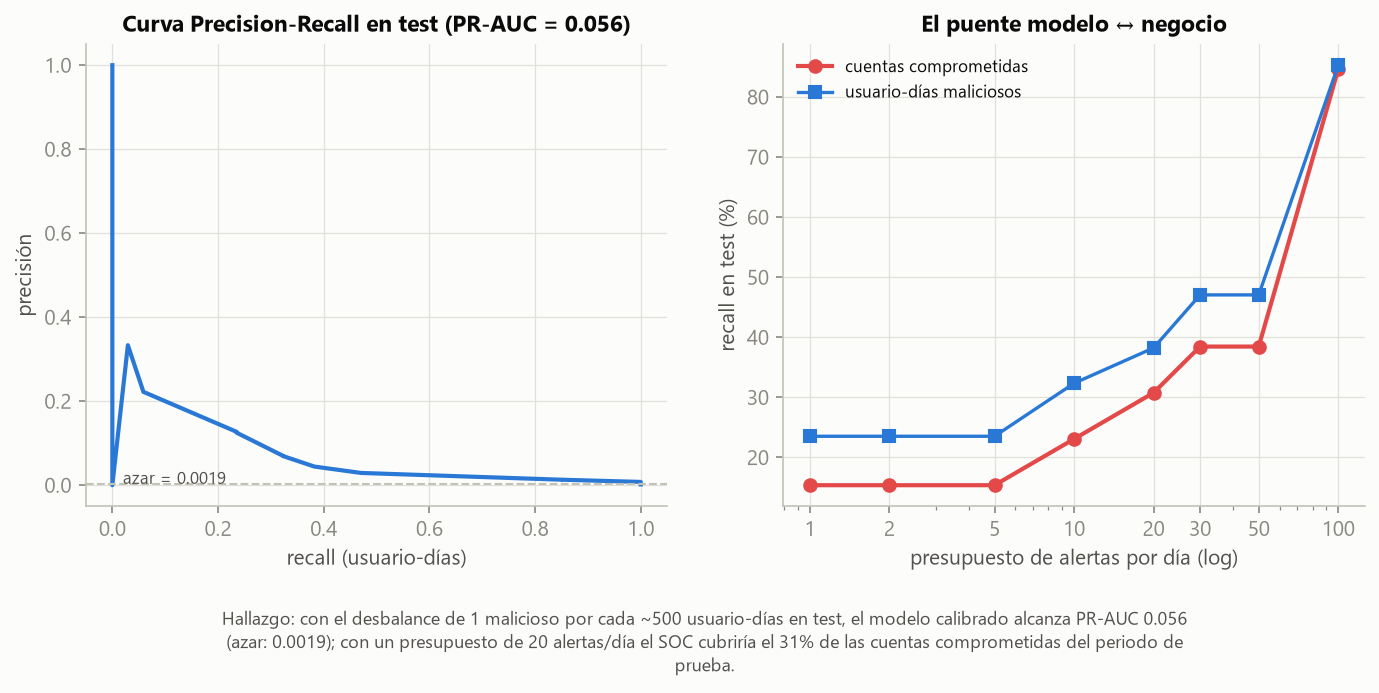
\includegraphics[width=\textwidth]{img/fig4_evaluacion.png}
  \caption{Izquierda: curva precisión-recall en prueba (la línea punteada es el azar). Derecha: el
  puente entre el modelo y el negocio ---recall de cuentas comprometidas en función del presupuesto
  de alertas por día.}
  \label{fig:eval}
\end{figure}

El panel derecho de la Figura~\ref{fig:eval} es, en mi opinión, la herramienta más valiosa para el
negocio, pues traduce el desempeño estadístico en lenguaje operativo: con un presupuesto de 20 alertas
diarias, el sistema cubre el 31\% de las cuentas comprometidas del periodo; con 100 alertas diarias,
el 85\%. Esta curva convierte la pregunta «¿qué tan bueno es el modelo?» en «¿cuántos analistas cuesta
cada punto de recall?».

\subsection{Reporte de estabilidad}

Un modelo que discrimina pero se desestabiliza entre periodos no es desplegable. Por ello incluí un
reporte de estabilidad sobre el periodo fuera de tiempo, con los indicadores estándar de la industria
del riesgo \cite{siddiqi2006}. El \textbf{PSI} (\textit{Population Stability Index}) de la puntuación
entre entrenamiento y prueba fue de 0.019, dentro del rango «estable»: la distribución de scores que
vería el SOC apenas se movió entre periodos. El estadístico \textbf{KS} de clasificación fue de 0.74,
indicando una separación fuerte entre las poblaciones de positivos y negativos. El \textbf{CSI}
(\textit{Characteristic Stability Index}) de las variables reveló que dos de ellas ---las
desviaciones de fallos y de NTLM respecto a los pares--- sí derivan entre periodos, lo cual no es un
defecto del \textit{pipeline} sino un hecho del fenómeno: ambas dependen de \textit{cómo} ataca el
\textit{red team} en cada campaña, que cambia. El resto de las variables, incluidas todas las de
grafo, permanecen estables, y el \textit{score} agregado se mantiene estable pese a la deriva de esas
dos entradas.

\subsection{Explicabilidad}

Cumpliendo el principio de diseño de que ninguna puntuación viaje sin su explicación, empleé valores
SHAP \cite{lundberg2017} para interpretar el modelo. El resumen global (Figura~\ref{fig:shap})
confirma que las señales dominantes son el ratio de NTLM, el número de máquinas origen nuevas y la
rareza media de los destinos ---es decir, protocolo anómalo y novedad de grafo, no volumen crudo. El
modelo aprendió la tesis del proyecto, no un atajo. Esta misma técnica, en su versión local por
usuario-día, es la que alimenta la explicación que el analista ve en la interfaz.

\begin{figure}[!htb]
  \centering
  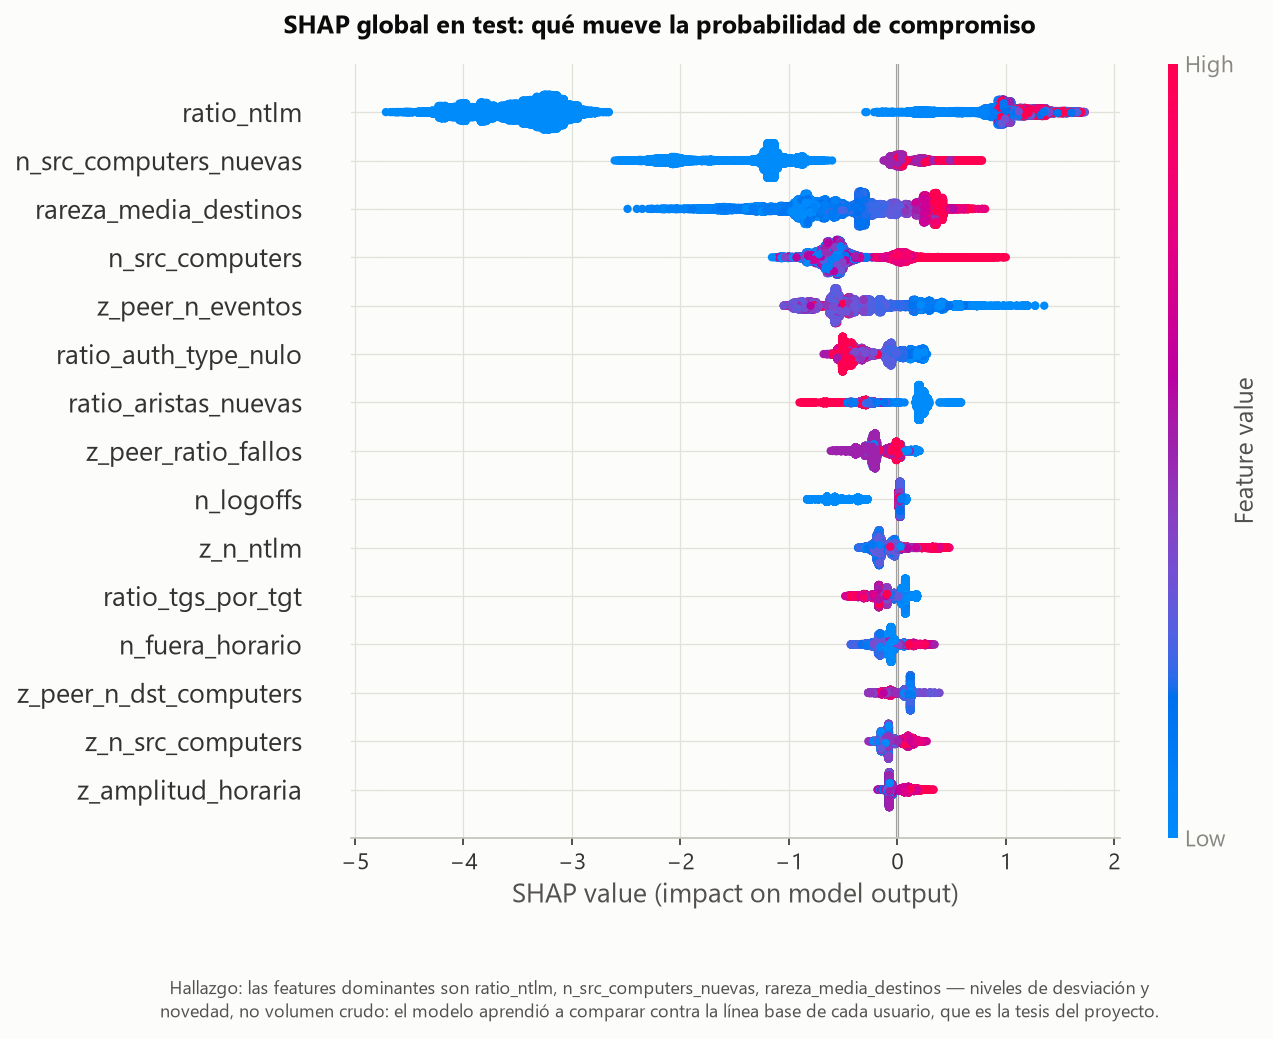
\includegraphics[width=0.95\textwidth]{img/fig5_shap_summary.png}
  \caption{Resumen global de valores SHAP sobre el conjunto de prueba. Dominan las variables de
  protocolo y de novedad de conexiones, validando el diseño multinivel de la ingeniería de variables.}
  \label{fig:shap}
\end{figure}

\FloatBarrier

% ────────────────────────────────────────────────────────────────────────────
\section{Análisis crítico y conflictos del desarrollo}

Considero que la honestidad sobre las limitaciones es parte del rigor científico, por lo que dedico
una sección al análisis crítico de los resultados y a los conflictos que enfrenté, más allá de los
ya narrados en la adquisición de datos y el agrupamiento degenerado.

\subsection{Tercer conflicto: una autocorrección metodológica}

Antes de aceptar los resultados como definitivos, exploré tres palancas para mejorarlos, y durante
esa exploración cometí ---y corregí--- un error metodológico que documento precisamente porque su
corrección es evidencia de rigor. Al probar la agregación del riesgo a nivel de cuenta (tomar el
máximo de los últimos $K$ días), inicialmente elegí $K=7$ porque era el valor que mejor se veía
\textit{en el conjunto de prueba}, obteniendo un PR-AUC aparentemente superior de 0.084. Esto es
exactamente la fuga metodológica que había estado combatiendo durante todo el proyecto: elegir un
hiperparámetro mirando el conjunto de prueba. Lo detecté, rehíce la selección eligiendo $K$
correctamente sobre la validación ---que resultó en $K=1$, es decir, sin agregación--- y el
«resultado» de mejora se desvaneció.

\subsection{La exploración honesta de mejoras}

Probé tres palancas y ninguna sobrevivió a una selección honesta: (1) extender la ventana temporal no
añade positivos, pues verifiqué que no existen ataques fuera de los días 1--29 en el conjunto
completo; (2) combinar las puntuaciones de XGBoost y K-Means no generaliza, pues el peso óptimo en
validación no transfiere a prueba; y (3) la agregación por cuenta, correctamente evaluada, no mejora.
Esto no es un fracaso del \textit{pipeline}: con solo 181 eventos de compromiso en todo el conjunto,
no hay margen estadístico para que el ajuste fino encuentre algo que generalice, y el techo de esta
fuente de datos con este enfoque ya se alcanzó.

\subsection{Contextualización honesta de los resultados}

Los resultados son modestos en términos absolutos pero defendibles como primera iteración de un
problema genuinamente difícil. Un análisis de \textit{bootstrap} sobre los 34 positivos de prueba
arroja un intervalo de confianza del 95\% para el PR-AUC de $[0.022, 0.146]$: amplio por el tamaño de
muestra, pero cuyo límite inferior sigue estando cerca de nueve veces por encima de un ordenamiento
aleatorio (cuyo PR-AUC medio medí en 0.0025). La afirmación «el modelo discrimina mejor que el azar»
es, por tanto, sólida y no frágil. La honestidad exige reconocer también el costo: al umbral operativo
naranja, la precisión es baja (13 verdaderos positivos frente a 280 falsos positivos), lo que refleja
el reto real de este desbalance. El punto de comparación correcto para juzgar el modelo no es un
umbral absoluto de «bueno», sino el \textit{lift} sobre el azar y la estabilidad del ordenamiento,
criterios bajo los cuales el sistema cumple.

% ────────────────────────────────────────────────────────────────────────────
\section{Resolución del problema}

La utilidad de un modelo se materializa únicamente cuando es accesible para su usuario final. Dediqué
la última parte del proyecto a convertir los modelos entrenados en un sistema operativo completo.

\subsection{Pipeline de inferencia y puntuación de riesgo}

Serialicé todos los artefactos ---el XGBoost calibrado, el Isolation Forest, el K-Means, los umbrales
y el explicador SHAP--- y construí el flujo de inferencia que convierte un usuario-día en una
decisión accionable. La puntuación de riesgo (0--100) sigue la fórmula híbrida
$\text{riesgo} = 100 \cdot (w \cdot p_{\text{sup}} + (1-w)\cdot a_{\text{norm}})$, donde $p_{\text{sup}}$
es la probabilidad calibrada y $a_{\text{norm}}$ la anomalía normalizada. En lugar de adoptar un peso
$w$ arbitrario, lo elegí en validación por PR-AUC, y el resultado ($w = 0.95$) confirma con
transparencia que el componente supervisado domina. Los niveles del semáforo los recalibré en el
espacio 0--100 según la capacidad operativa del SOC.

\subsection{Consumo de modelos: la API}

Expuse los modelos mediante una API construida con FastAPI, que sirve una instantánea precomputada
del periodo de prueba a través de ocho \textit{endpoints} tipados: los indicadores generales, la cola
de triaje priorizada, la serie temporal de riesgo por usuario, la explicación SHAP con comparativas,
el resumen de actividad, el registro de decisiones del analista y un \textit{endpoint} de inferencia
en vivo. La API es la dueña de todo el conocimiento del modelo; el contrato queda documentado
automáticamente mediante OpenAPI, y validé su comportamiento con una suite de 23 pruebas de contrato.

\subsection{La interfaz de usuario}

Desarrollé la interfaz con React (mediante Vite y TypeScript), desplegada en producción, con tres
vistas que atienden a los tres perfiles de usuario: una \textbf{consola de triaje} con la cola
priorizada, la evolución del riesgo y la explicación SHAP; una vista de \textbf{investigación} que
incluye el mini-grafo ego que hace visible el movimiento lateral y el historial de decisiones; y un
\textbf{panel ejecutivo} con la tendencia de riesgo por rol conductual y la eficiencia del SOC. Un
principio gobernó todo el frontend: la interfaz nunca recalcula el riesgo; si un número no proviene de
la API, no existe.

\subsection{Asistente conversacional}

Como componente adicional de usabilidad, integré un asistente conversacional que responde preguntas
del usuario en lenguaje natural y sirve de guía. Lo implementé con la técnica de
\textit{function calling}: el modelo de lenguaje, cuando necesita un dato, invoca herramientas que
consultan la instantánea real del modelo, de modo que responde con las cifras verdaderas del periodo
en lugar de inventarlas. Por seguridad, la clave de la API del proveedor reside exclusivamente en el
servidor y nunca se expone al navegador.

% ────────────────────────────────────────────────────────────────────────────
\section{Conclusiones}

Este proyecto me permitió recorrer el ciclo completo de un problema de ciencia de datos aplicado a un
dominio real y difícil, desde mil millones de eventos crudos hasta una interfaz funcional en
producción. Organizo las conclusiones en tres planos: los hallazgos del análisis, el impacto para la
toma de decisiones y la justificación de las decisiones metodológicas de fondo.

\subsection{Hallazgos sobre el problema}

El hallazgo que considero más relevante, y que atraviesa todo el trabajo, es que la señal del uso
indebido de credenciales vive en la \textbf{desviación} y en la \textbf{novedad de conexiones}, no en
el volumen de actividad. El análisis SHAP lo confirmó de manera independiente: las variables
dominantes son el protocolo anómalo y las máquinas nuevas, no cuántos eventos genera el usuario. El
caso que analicé en detalle lo resume con precisión: el día del ataque, el volumen de esa cuenta
estaba dentro de lo normal (0.69 desviaciones estándar respecto a su propia media) mientras su
alcance estaba a 7.7 desviaciones. Un detector basado en volumen no habría visto nada.

Este resultado valida el diseño multinivel de la ingeniería de variables y, sobre todo, valida la
premisa de negocio: un sistema que vigile umbrales absolutos de actividad fracasará frente a un
atacante que opera dentro de una cuenta legítima.

\subsection{Hallazgos sobre los datos}

Tres resultados empíricos que no anticipaba al comenzar y que documento porque cambiaron decisiones
concretas del proyecto:

\begin{enumerate}[leftmargin=1.5cm]
  \item \textbf{El ritmo humano de la red puede recuperarse de tiempos completamente anónimos.}
        Únicamente a partir de la periodicidad de los datos inferí el horario laboral (7:00--16:00)
        y los fines de semana, sin ningún calendario externo. Un matiz metodológico importante:
        existe una base de automatización 24/7 corriendo bajo cuentas de usuario, de modo que el
        umbral correcto es el punto medio entre valle y pico; usar un porcentaje del pico habría
        clasificado el día entero como laboral.
  \item \textbf{El compromiso no se parece a la fuerza bruta.} Los días comprometidos presentan
        fallos con más frecuencia (50\% de los días frente a 24\%) pero en proporción mínima (ratio
        típico de 0.003), porque quien usa credenciales válidas robadas avanza con éxito. El fallo
        masivo pertenece a la población normal: el 17\% de los usuario-días normales son 100\%
        fallos, la firma de automatización con credenciales caducas. A nivel de evento, el
        \textit{red team} autenticó con éxito el 99.9\% de las veces. Esta observación invirtió mi
        expectativa inicial y obligó a contextualizar la variable de fallos contra el historial del
        propio usuario en lugar de usarla en crudo.
  \item \textbf{La variable de identidad destino resultó de las más discriminantes.} El número de
        veces que una cuenta aparece como identidad \textit{destino} de otra ---que añadí casi por
        completitud--- separa las clases con una mediana de 20 frente a 0. Es la firma de las cadenas
        de saltos entre máquinas.
\end{enumerate}

\subsection{Impacto para la toma de decisiones}

El valor del sistema no reside en una métrica sino en la curva que traduce el modelo a capacidad
operativa. La Tabla~\ref{tab:negocio} resume esa traducción.

\begin{table}[!htb]
\centering
\small
\setlength{\tabcolsep}{8pt}
\begin{tabular}{cc}
\toprule
\textbf{Presupuesto de alertas diarias} & \textbf{Cobertura de cuentas comprometidas} \\
\midrule
20 alertas / día  & 31\% \\
30 alertas / día  & 38\% \\
50 alertas / día  & 38\% \\
100 alertas / día & \textbf{85\%} \\
\bottomrule
\end{tabular}
\caption{Traducción del desempeño estadístico a capacidad operativa. Permite a un responsable de
seguridad elegir su punto de operación en función del equipo disponible.}
\label{tab:negocio}
\end{table}

Esta tabla convierte una pregunta técnica ---«¿qué tan bueno es el modelo?»--- en una que una
dirección puede responder: \textbf{«¿cuántos analistas cuesta cada punto de cobertura?»}. En lugar de
imponer un umbral, el sistema permite elegir el punto de operación según los recursos reales.

También es necesario ser explícito sobre el costo. Al umbral naranja la precisión es baja: 13
aciertos frente a 280 falsos positivos. Presentado de forma aislada el dato suena descalificador,
pero el marco correcto es otro: el sistema reduce 17\,501 usuario-días a 212 casos revisables, y
dentro de esa lista corta el analista descarta con rapidez gracias al semáforo y la explicación. Es
una herramienta de \textbf{priorización}, no de bloqueo automático, y por eso ninguna acción sobre
una cuenta ocurre sin decisión humana.

Conviene subrayar además el encaje del producto: Nexus Sentinel no compite con el SIEM ni con el
EDR, sino que consume sus registros y devuelve priorización explicada. Es exactamente la capa que
faltaba en incidentes como el de Target, donde las alertas técnicas existían pero se perdieron entre
el ruido porque nadie podía distinguir cuáles merecían atención.

\subsection{Justificación del enfoque supervisado}

La elección del aprendizaje supervisado como componente central está sólidamente justificada para
este problema. Dado que dispongo de etiquetas verificadas del \textit{red team}, puedo optimizar
directamente la función objetivo del negocio y medir el desempeño de forma objetiva, algo que un
enfoque puramente no supervisado ---que solo identificaría desviaciones estadísticas sin distinguir
compromiso genuino de comportamiento legítimo atípico--- no permitiría.

No obstante, integré ambos paradigmas y ambos aportaron. El Isolation Forest actúa como línea base
que contextualiza el desempeño del modelo central, y el agrupamiento de pares cumple un doble papel:
genera las variables de desviación grupal ---que resultaron valiosas en el análisis SHAP--- y, como
puntuación de anomalía por distancia al centroide, superó a la línea base con un modelo mucho más
simple (PR-AUC de 0.093 frente a 0.027).

\subsection{Sobre el rigor metodológico}

Valoro especialmente que los conflictos que enfrenté ---el \textit{data fence} en la adquisición, el
agrupamiento degenerado y, sobre todo, la autocorrección de la fuga metodológica--- no fueran
obstáculos que ocultar, sino oportunidades para demostrar el rigor con el que abordé el trabajo.

Si tuviera que quedarme con una sola idea del proyecto, sería que \textbf{la honestidad metodológica
es parte del resultado}. Documenté el agrupamiento que tuve que corregir, la fuga que yo mismo
introduje y detecté, las tres palancas de mejora que no funcionaron y la tasa de falsos positivos sin
filtrar. Un modelo con métricas modestas pero verificables y estables vale más que uno con números
vistosos que no resistirían escrutinio; y en seguridad, donde las decisiones afectan a personas, esa
diferencia es la que importa.

% ────────────────────────────────────────────────────────────────────────────
\section{Limitaciones y recomendaciones}

\subsection{Limitaciones del trabajo}

Prefiero enunciarlas explícitamente antes que dejar que las descubra quien evalúe el proyecto:

\begin{itemize}[leftmargin=1.5cm]
  \item \textbf{El volumen de positivos marca el techo.} Con 181 eventos de compromiso en todo el
        conjunto (120, 27 y 34 por partición), el margen estadístico es estrecho. Probé tres palancas
        de mejora y ninguna sobrevivió a una selección honesta en validación.
  \item \textbf{Dos variables derivan entre campañas.} Las desviaciones de fallos y de NTLM respecto
        a los pares presentan un índice de estabilidad alto, porque dependen de \textit{cómo} ataca
        el equipo ofensivo en cada campaña. La puntuación agregada se mantiene estable, pero esas dos
        variables requerirían monitoreo en un despliegue real.
  \item \textbf{La fuente tiene un sesgo conocido.} El conjunto solo incluye fallos de autenticación
        de usuarios que tuvieron al menos un éxito, de modo que los ataques de adivinación contra
        cuentas inexistentes quedan fuera del alcance por construcción. No es corregible: son
        registros que no existen.
  \item \textbf{El ROC-AUC de 0.939 es engañoso} con este desbalance, razón por la cual lo reporto
        siempre acompañado de la curva de precisión-recall.
  \item \textbf{La inferencia opera sobre variables precomputadas}, no sobre eventos crudos en
        caliente. La reconstrucción completa desde eventos reutilizaría los mismos módulos, pero
        requeriría transmitir el estado histórico de cada usuario.
\end{itemize}

\subsection{Recomendaciones y trabajo futuro}

Ordeno las líneas de continuación por la relación entre impacto esperado y esfuerzo requerido:

\begin{enumerate}[leftmargin=1.5cm]
  \item \textbf{Enriquecer con fuentes de datos adicionales.} Es la única palanca que añadiría
        \textit{señal nueva} en lugar de reordenar la existente, y por eso la sitúo en primer lugar.
        El propio conjunto de LANL incluye eventos de procesos y flujos de red que no utilicé. Un
        proceso inusual ejecutándose en una máquina recién alcanzada constituye evidencia
        independiente del movimiento lateral, y combinarla con la novedad de grafo debería mejorar la
        precisión justamente donde más importa: en la cabeza de la cola de triaje.
  \item \textbf{Cerrar el ciclo de retroalimentación.} La interfaz ya registra las decisiones del
        analista (falso positivo, investigar, escalar). Con suficientes decisiones acumuladas, esas
        etiquetas humanas permitirían reentrenar el modelo sobre lo que el equipo considera realmente
        relevante, que no siempre coincide con la definición del \textit{red team}.
  \item \textbf{Recalibrar los umbrales periódicamente.} Observé que el volumen de alertas se
        desplaza ligeramente entre periodos. En operación, los percentiles deberían recalcularse
        sobre una ventana móvil reciente en lugar de quedar fijos, de modo que la carga diaria se
        mantenga dentro de la capacidad del equipo.
  \item \textbf{Convertir el análisis de estabilidad en monitoreo continuo.} Los índices PSI y CSI
        que calculé no deberían ser un ejercicio único: automatizados, permitirían detectar cuándo el
        modelo necesita reentrenarse porque el comportamiento de la red cambió.
  \item \textbf{Explorar modelos de secuencia.} La unidad usuario-día resume una jornada completa en
        una fila. Modelos que traten la secuencia de eventos dentro del día podrían capturar el
        \textit{orden} del movimiento lateral, no solo su magnitud. Lo sitúo al final
        deliberadamente: con 181 positivos, un modelo de mayor capacidad probablemente sobreajustaría,
        de modo que esta línea solo tiene sentido después de ejecutar la primera.
\end{enumerate}

% ────────────────────────────────────────────────────────────────────────────
\section{Referencias}

\renewcommand{\refname}{}
\begin{thebibliography}{11}

\bibitem{verizon2024}
Verizon. (2024). \textit{2024 Data Breach Investigations Report (DBIR)}. Verizon Business.
\url{https://www.verizon.com/business/resources/reports/dbir/}

\bibitem{kent2015data}
Kent, A. D. (2015). \textit{Comprehensive, Multi-Source Cyber-Security Events} [Data set]. Los Alamos
National Laboratory. \url{https://csr.lanl.gov/data/cyber1/}

\bibitem{kent2015book}
Kent, A. D. (2015). Cybersecurity Data Sources for Dynamic Network Research. En \textit{Dynamic
Networks and Cyber-Security}. Imperial College Press.

\bibitem{liu2008}
Liu, F. T., Ting, K. M., \& Zhou, Z.-H. (2008). Isolation Forest. \textit{Proceedings of the 2008
Eighth IEEE International Conference on Data Mining (ICDM)}, 413--422.

\bibitem{chen2016}
Chen, T., \& Guestrin, C. (2016). XGBoost: A Scalable Tree Boosting System. \textit{Proceedings of the
22nd ACM SIGKDD International Conference on Knowledge Discovery and Data Mining}, 785--794.

\bibitem{lundberg2017}
Lundberg, S. M., \& Lee, S.-I. (2017). A Unified Approach to Interpreting Model Predictions.
\textit{Advances in Neural Information Processing Systems (NeurIPS)}, 30, 4765--4774.

\bibitem{macqueen1967}
MacQueen, J. (1967). Some Methods for Classification and Analysis of Multivariate Observations.
\textit{Proceedings of the Fifth Berkeley Symposium on Mathematical Statistics and Probability}, 1,
281--297.

\bibitem{rousseeuw1987}
Rousseeuw, P. J. (1987). Silhouettes: A Graphical Aid to the Interpretation and Validation of Cluster
Analysis. \textit{Journal of Computational and Applied Mathematics}, 20, 53--65.

\bibitem{saito2015}
Saito, T., \& Rehmsmeier, M. (2015). The Precision-Recall Plot Is More Informative than the ROC Plot
When Evaluating Binary Classifiers on Imbalanced Datasets. \textit{PLoS ONE}, 10(3), e0118432.

\bibitem{siddiqi2006}
Siddiqi, N. (2006). \textit{Credit Risk Scorecards: Developing and Implementing Intelligent Credit
Scoring}. John Wiley \& Sons. (Referencia para los índices de estabilidad PSI, CSI y el estadístico KS.)

\bibitem{mitre}
The MITRE Corporation. (2023). \textit{MITRE ATT\&CK: Lateral Movement (TA0008) y Use Alternate
Authentication Material: Pass the Hash (T1550.002)}. \url{https://attack.mitre.org/}

\end{thebibliography}

\end{document}
